\section{Конечные автоматы}

\subsection{Конечные детерменированные автоматы}

Конечным детерменированным автоматом 
называется пятерка объектов $A = (S, X, Y, \delta, \lambda)$, где
$S$, $X$, $Y$ "--- конечные непустые множества, 

$S$ "--- множество состояния
автомата, а его элементы "--- состояния автомата.

$X$ "--- входной алфавит(множество входных сигналов).

$Y$ "--- выходной алфавит(множество выходных сигналов).

$\delta$ и $\lambda$ "--- функции переходов и выходов:

\begin{equation*}
    \delta: ~ S \times X \rightarrow S
\end{equation*}

\begin{equation*}
    \lambda: ~ S \times X \rightarrow Y
\end{equation*}

Автомат работает в дискретной временной шкале(в моменты времени $t_i \in \mathbb{N}$)
и в зависимости от того, в каком состоянии $S$ и какой сигнал $x \in X$ он получает, 
в следующий момент времени $t_{i+1}$ он перейдет в состояние $\delta(S, x)$ и
будет получено $\lambda(S, x)$ на выходе.

\subsection{Способы задания автоматов}

Автоматы можно задавать с помощью таблицы переходов-выходов или в виде
графа.

Рассмотрим эти способы.

\subsubsection{Таблица переходов автоматов}

Строки представляют из себя состояния автоматов, а столбцы "--- слова из множества $X$.

\begin{figure}[h!]
    \centering
    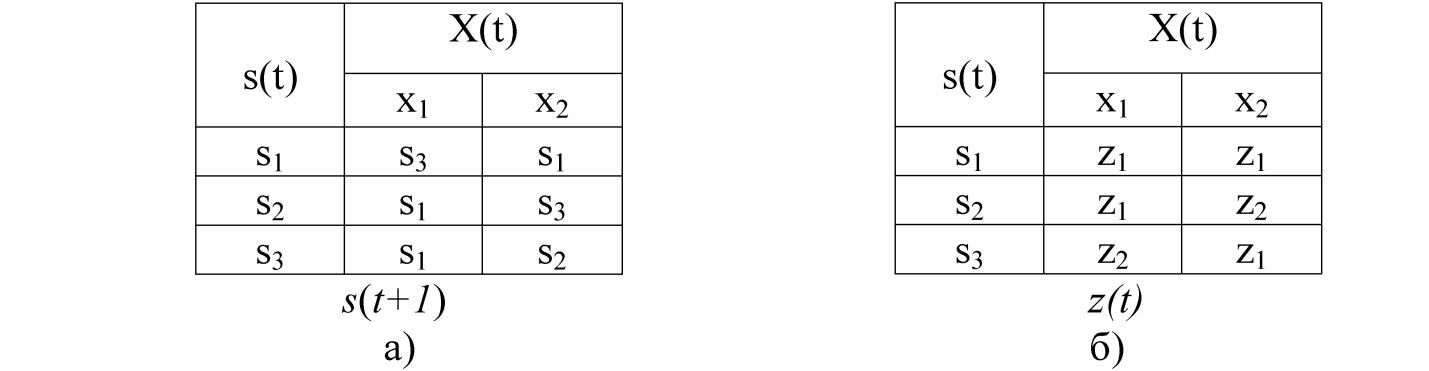
\includegraphics[scale=0.7]{table.png}
    \caption{Таблица переходов-выходов}
\end{figure}

\subsubsection{Граф автомата}

Вершинами являются элементы множества состояний, а ребра представляют из себя
пару элементов $(x,y) ~|~ x \in X, y \in Y$.


\begin{figure}[H]
    \centering
    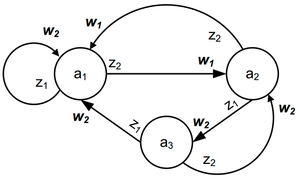
\includegraphics[scale=0.7]{graph.png}
    \caption{Граф автомата}
\end{figure}

Вершины "--- элементы множества состояний.

$\varepsilon$ "--- пустая цепочка (слово, которое не содержит ни одной буквы).

$|\varepsilon| = 0$


\begin{definition}
    Алфавитом назовем любое конечное непустое множество.
\end{definition}

\begin{definition}
    Словом над алфавитом $M$ назовем любую последовательность $p$ $x_1 x_2 \dots x_n$ такую, что
    $x_i \in M$. Если $p$ "--- слово над $M$, то длиной слова назовем количество
    букв этого слова и обозначим его как $|p|$.
\end{definition}

\begin{definition}
    Множество всех слов над алфавитом $M$ длины $k$ будем обозначать как $M^k$
\end{definition}

\begin{definition}
    Пусть $A(S, X, Y \delta, \lambda)$ "--- конечный детерменированный автомат.
    Продолженные (расширенные) функции переходов и выходов на слова входного
    алфавита $X$ определим индуктивно:
    
    $\delta(s, \varepsilon) = s$, $\delta(s, px) = \delta(\delta(s, p), x)
    ~\forall s \in S , ~p \in X^* ,~ x \in X$
\end{definition}

% Добавить примеры

\begin{definition}
    Два автомата $A_1$ и $A_2$ называются сравнимыми, если у них одинаковый
    входной и выходной алфавиты.
\end{definition}

\begin{definition}
    Будем говорить, что $A_1(S_1, X_1, Y_1, \delta_1, \lambda_1$ изоморфен
    автомату $A_2(S_2, X_2, Y_2, \delta_2, \lambda_2)$, если существует
    тройка биекций:
    \begin{equation*}
        \phi : ~ S_1 \rightarrow S_2
    \end{equation*}
    \begin{equation*}
        \psi : ~ X_1 \rightarrow X_2
    \end{equation*}
    \begin{equation*}
        \xi : ~ Y_1 \rightarrow Y_2
    \end{equation*}
    удовлетворяющая следующему условию:
    \begin{equation*}
        \forall s \in S_1, x \in X_1 : ~ \phi(\delta_1(s, x)) = \delta_2(\phi(s), \psi(x))
    \end{equation*}
    \begin{equation*}
        \forall s \in S_1, x \in X_1 : ~ \xi(\lambda_1(s, x)) = \lambda_2(\phi(s), \psi(x))
    \end{equation*}
\end{definition}

% Добавить рисунок


\begin{definition}
    Пусть $A_1$, $A_2$ "--- сравнимые автоматы. $A_1 \simeq A_2$, если
    $\exists \psi: ~ S_1 \rightarrow S_2$, что выполняется

    \begin{equation*}
        \forall s \in S, x \in X:~ \begin{matrix}
             \phi(\delta_1, (s, x)) = \delta_2(\phi(s), x) \\
             \lambda_1(s, x) = \lambda_2(\phi(s), x)
        \end{matrix}
    \end{equation*}
\end{definition}

\begin{theorem}[Об изоморфизме автоматов]
    Отношение изоморфизма на множестве всех автоматов есть отношение эквивалетности.
\end{theorem}

\begin{proof}
    Докажем, что для этого отношения характерны свойства отношения эквивалентности
    \begin{enumerate}
        \item Рефлексивность.
        
        $\begin{matrix}
            \phi : S_1 \rightarrow S_2 \\
            \psi : X_1 \rightarrow X_2 \\
            \xi : Y_1 \rightarrow Y_2 \\
        \end{matrix}$

        Покажем, что $\forall s \in S, x \in X$ выполняется

        \begin{equation*}
            \begin{matrix}
                \phi(\delta_1(s, x)) = \delta_2(\phi(s), \psi(x)) \\
                \xi(\lambda_1(s, x)) = \lambda_2(\phi(s), \psi(x))
            \end{matrix}
        \end{equation*}
            $\forall x \in X, y \in Y, s \in S: ~~~
            \begin{matrix}
                \phi(s) = s \\
                \psi(x) = x \\
                \xi(y) = y  
            \end{matrix} $

        Тогда 
        \begin{equation*}
            \begin{matrix}
                \phi(\delta(s, x)) = \delta(s, x) = \delta(\phi(x), \psi(s)) \\
                \xi(\lambda(s, x)) = \lambda(s, x) = \lambda(\phi(x), \xi(s))
            \end{matrix}
        \end{equation*}
        \item Симметричность.
        % TODO
    \end{enumerate}
\end{proof}


\paragraph{Утверждение}





